% !TEX root = ./main.tex

\section{Methods}

\textbf{Molecular Dynamics}

Molecular simulation trajectories of \emph{ab initio} peptide binding
were performed on Folding@home (FAH) (7) using Gromacs 4.5.4 (8) with
TIP3P explicit solvent and the Amber ff99sb-ildn-nmr force field, as
described by Zhou et al (1). The protein data bank (PDB) denotes the
well-known MDM2-p53 system as 1YCR. Initial atomic coordinates from 1YCR
were used as a template in the production of approximately 976 µs of
aggregate simulation data.

\textbf{Solvent Shell Featurization}

Previously, the analysis of trajectories consisted of strictly protein
conformational degrees of freedom (DOF). Pair distance features between
C\textsubscript{α} and C\textsubscript{β} atoms of selected residues
(see Supplementary Materials) positioned within the binding region of
MDM2 and p53 were used. In contrast to the distance metric between
C\textsubscript{α} and C\textsubscript{β} atoms in Zhou's work, each
trajectory was described by the "SolventShellFeaturizer'' tool for
MSMBuilder (9).

Solvent features are a collection of all the water oxygens that had been
binned in accordance to their respective shell occupancies.
``Important'' water atoms are defined as the solvent atoms located in
the union of two or more shells with differing solute atoms. Parameters
for the solvent shell featurization followed the optimization determined
by Harrigain et al., (9) which encompasses the use of four solvent
shells around each solute atom with a shell width equal to 3.0 Å each.

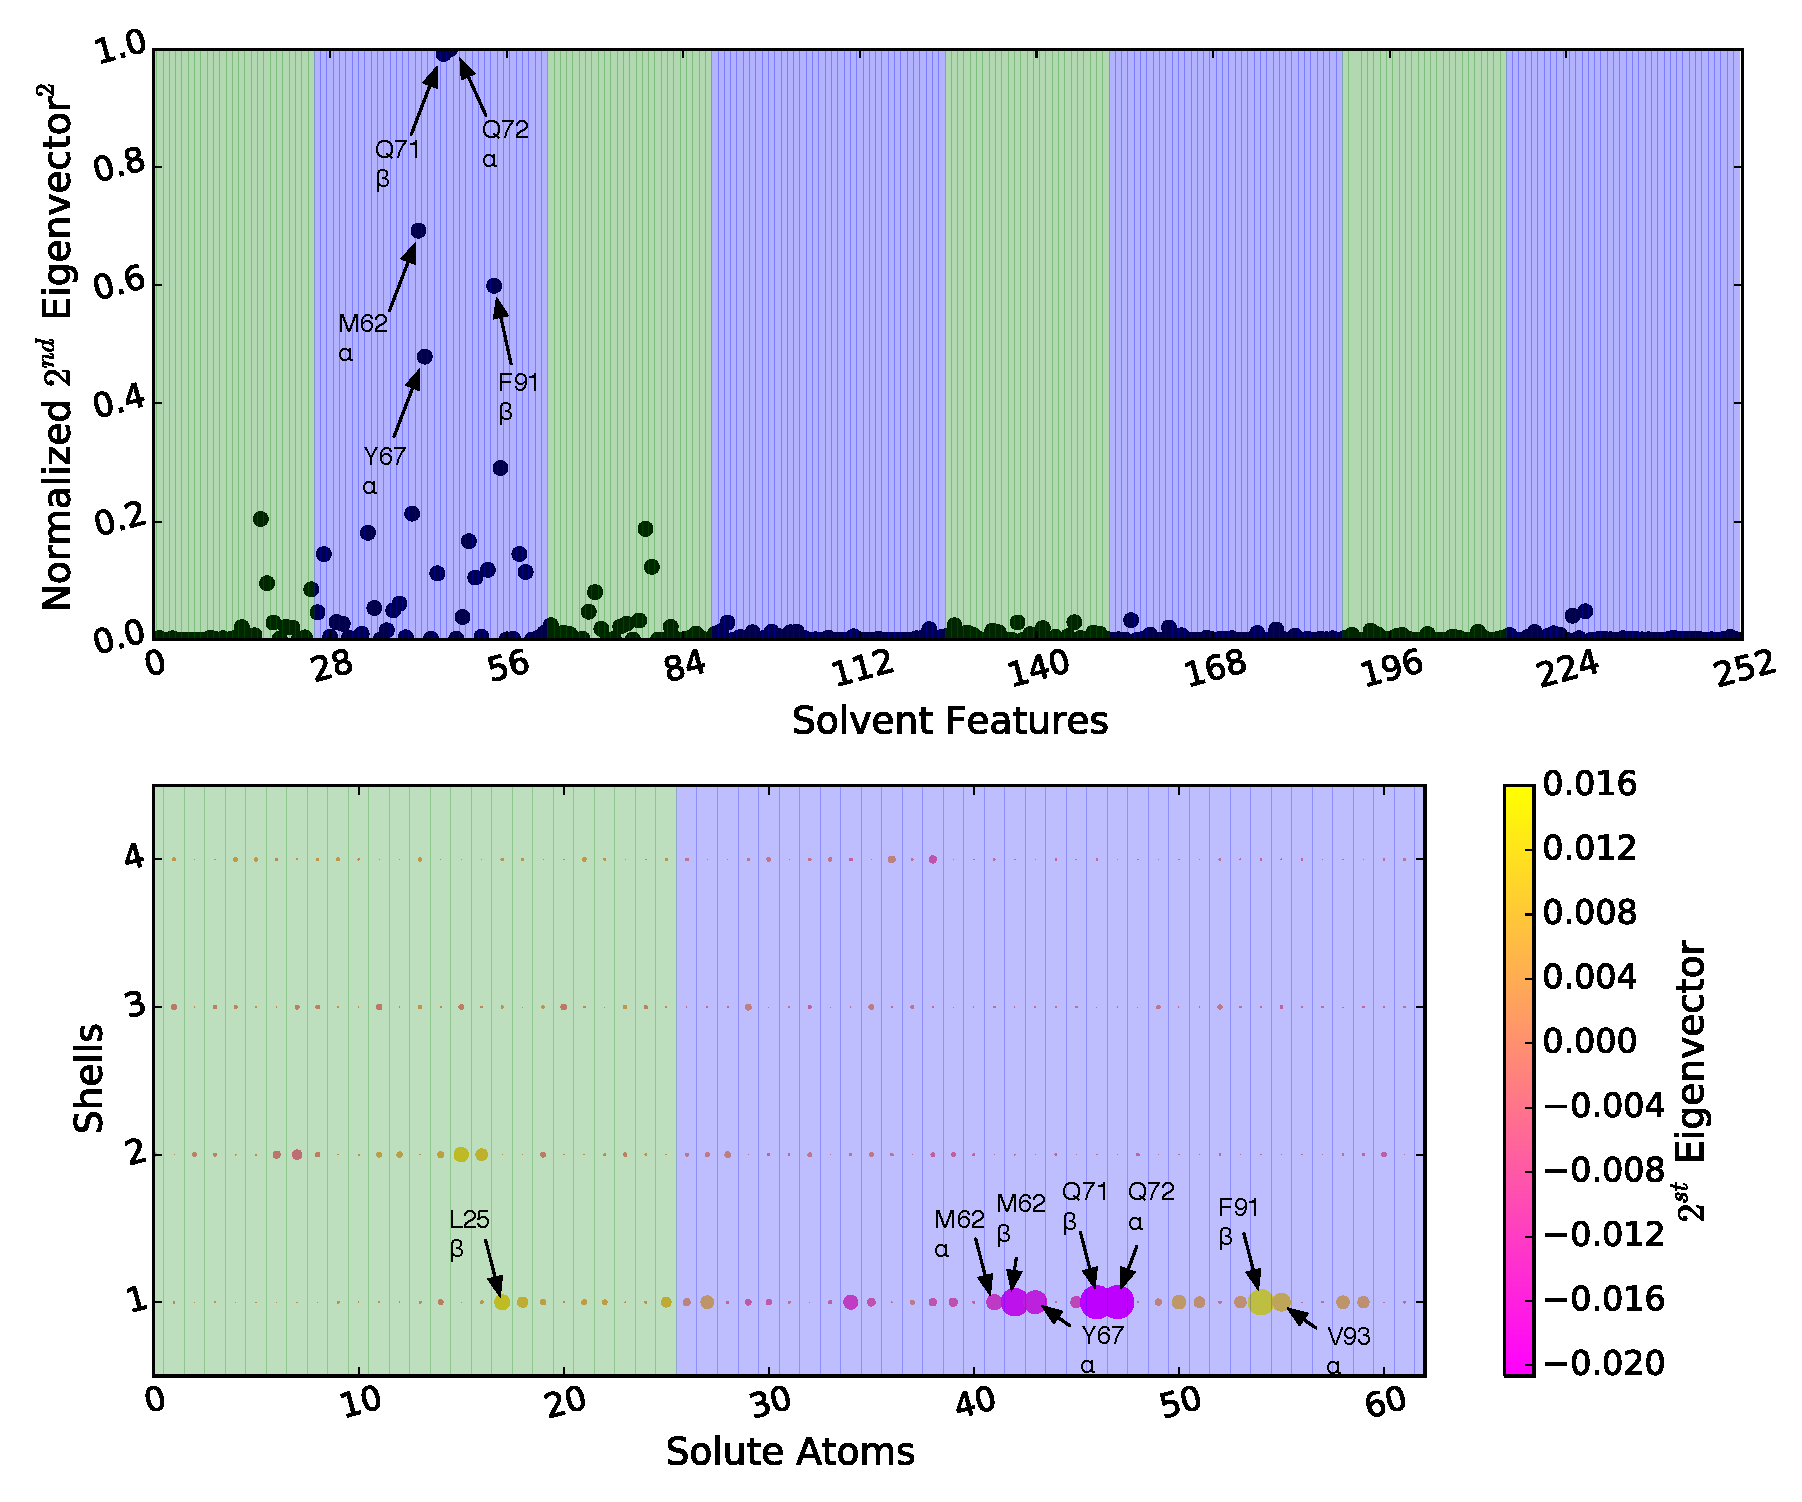
\includegraphics[width=6.5in,height=2.29097in]{media/image1.emf}

\textbf{Figure 1.} "Solvent Shell Featurization" provides location of
specific solvent shell features by binning solvent atoms (blue circles)
according to specific solute atoms (green circles) with respect to shell
index. ``Important'' solvent features are highlighted red, which are
defined by solvent atoms residing within overlapping shells (gray
shading).

\textbf{MSM construction}

In recent years, MSMs have proven to proven to be a strong tool in many
sectors of biophysics, including protein folding (10, 11),
conformational dynamics (1), as well as solvent dynamics (9). We
describe solvent dynamics using WetMSM (9), MDTraj (12) and MSMbuilder
(13) libraries. Using the latter python libraries, linear combinations
of solvent features were used to compute a new basis set, the tICA
subspace. The eigenvectors of the tICA time-correlation matrix relate to
the degrees of freedom associated with the conformational change (6).
Hence, the metastability of specific solvent shells contributing to the
slowest de-wetting processes were determined from the eigenvectors
correlated with the slowest relation timescales.

Previous tests suggest (14) that 10 tICA components with 600 microstates
and a 5 ns lagtime is best suited for the construction of the
protein-only tICA model. In order to compare protein and solvent MSM's,
the tICA parameters remained the same in the wetMSM (9) construction.

\textbf{MolMap }

Chimera's molmap (16) function allows for visualization of specific
water density within trajectories. Appling this volume density map
technique provides an unparalleled visualization of ``important''
solvent-protein interactions. All water-oxygens for each snapshot were
selected when computing the density surface. The initial contour level
to enclose a fraction of the total mass was set to 0.9895 and the grid
spacing to 1.3. The volume contour level was then changed to 0.015 to
apply Gaussian filtering. Gaussian filtering was performed for each
individual surface in order to reduce the amount of flickering when
moving from snapshot to snapshot.


